\section{Экспериментальная проверка и анализ результатов}

TODO2

\subsection{Результаты обучения классификаторов и сегментаторов}

Ряд экспериментов подтвердил, что задача является решаемой. В частности, показатели обучения имеют стабильное, типовое поведение для подобных задач:

\begin{figure}
    \centering
    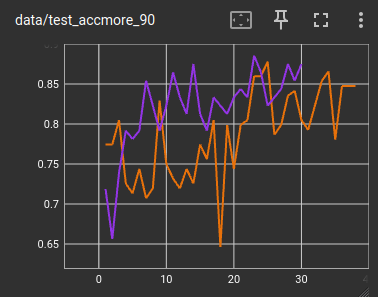
\includegraphics[width=0.5\linewidth]{figures/plot_cls_acc_1.png}
    \caption{График зависимости точности работы классификатора на тестовой выборке обучения от эпохи (bossExtrusion-оранжевый, fillet-фиолетовый)}
    \label{fig:placeholder}
\end{figure}

\begin{figure}
    \centering
    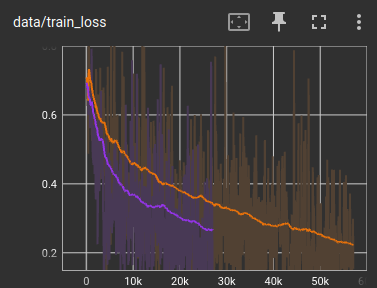
\includegraphics[width=0.5\linewidth]{figures/plot_cls_loss_1.png}
    \caption{График зависимости ошибки классификатора на обучающем датасете от эпохи обучения (bossExtrusion-оранжевый, fillet-фиолетовый)}
    \label{fig:placeholder}
\end{figure}

график accmore\_90 (Рисунок 4а) - показывает точность предсказания нейронной сети на тестовой выборке, чем больше значение - чем точнее предсказания; в случае успешного обучения, должен быть виден тренд на увеличение, что и происходит на картинке.
график train\_loss (Рисунок 4б) - показывает функцию ошибки на обучающем датасете, чем меньше значение - тем лучше обучена нейросеть; в случае успешного обучения, данный график должен стремиться к 0, что и происходит на картинке;
Таким образом, получено базовое подтверждение возможности использования STEP и текстового формата JSON для обучения нейросетей, так как обнаружен статистически извлекаемый сигнал: геометрия и последовательности операций содержат информацию, пригодную для машинного обучения и распознавания информации о типе операции.


После обучения в течение 50 эпох на датасете, полученном после очищения 21 464 моделей, получены следующие значения метрик:

\begin{table}[h]
\centering
\caption{Результаты сегментации}
\label{tab:segmentation-results}
\begin{tabular}{|l|c|c|c|}
\hline
\textbf{Операция} & \textbf{Доля верно определённых классов} & \textbf{Доля моделей, определённых на $\geq$90\%} & \textbf{Исходное распределение классов} \\
\hline
bossExtrusion & 78.4\% & 46.8\% & 59\% / 41\% \\
\hline
cutExtrusion (curve) & 96.8\% & 91.3\% & 56\% / 44\% \\
\hline
fillet & 93.6\% & 78.7\% & 40\% / 60\% \\
\hline
chamfer & 68.1\% & 53.125\% & 53\% / 47\% \\
\hline
\end{tabular}
\end{table}

“доля верно определённых классов” - число, равное отношению количества верно предсказанных классов рёбер к общему числу рёбер во всех моделях (сегментация), или отношению верно определённых наличия операции в модели с уверенностью выше 50\% к общему числу моделей (классификация);
“доля моделей, определённых на >=90\%” - число, равное количеству моделей, в которых 90\% всех рёбер были верно проклассифицированы;
“исходное распределение классов” - отношение количества классов в датасете (первое число - сколько рёбер / моделей соответствуют текущей операции, второе - сколько не соответствуют).
Все операции показали статистически значимое улучшение над тривиальной стратегией постоянного угадывания доминирующего класса. Это означает, что сеть научилась распознавать не только наиболее массовую операцию, но и часть остальных операций. Следует подчеркнуть, что данный результат нельзя без дополнительных проверок интерпретировать как достаточный уровень качества, в частности ввиду использования различных датасетов под каждую операцию в связи с её спецификой. Это содержательный baseline. Он показывает, что выбранная постановка для классификации операций дает сигнал выше случайного и выше простого частотного базиса. На данной стадии проекта это позволяет обоснованно переходить к улучшению и расширению датасетов и моделей.



\subsection{Анализ типовых ошибок и способов их устранения}

Этап 3 дал более содержательное качественное знание: было показано, что архитектуры на основе point cloud и DGCNN/LSTM-подобных блоков способны генерировать структурированное представление операции, но регрессионная часть остается ограничивающим фактором. В инженерной интерпретации это означает, что сеть понимает «что произошло», но недостаточно надежно восстанавливает «точно как именно это было задано численно». Такой результат дал проекту главное основание для корректной смены постановки.

Для сегментационного подхода наиболее конкретной зафиксированной метрикой является предварительная точность 84,5\% на тестовой выборке по операции fillet. Необходимо подчеркнуть несколько обстоятельств. Во-первых, это результат специализированного эксперимента, а не итоговая интегральная точность всей системы по всем операциям. Во-вторых, обучение проводилось на 1 726 моделях после дополнительных ограничений по сложности геометрии. В-третьих, метрика отражает точность предсказания типов ребер или элементов в задаче локальной сегментации, а не полноту восстановления дерева построения. Тем не менее именно этот результат является наиболее сильным количественным подтверждением правильности нового направления.

По результатам этапа также были определены косвенные признаки адекватности обучения: рост точности на тестовой выборке и убывание функции потерь на обучающей выборке без явных признаков немедленного переобучения. Для исследовательского этапа это важно, поскольку показывает, что модель продолжает извлекать информацию из данных и не исчерпала полезную емкость текущей выборки. Также был сделан вывод о необходимости более длительного обучения, а также о целесообразности дальнейшего расширения обучающего массива.

В то же время ряд примеров демонстрирует типичные ошибки. На одной из визуализаций отверстия ошибочно определяются как скругления; на другой видны отдельные ложноположительные ребра. Эти ошибки содержательно понятны. Геометрические признаки отверстий и скруглений частично пересекаются, особенно если рассматривать только локальные участки сетки без широкого контекста; небольшое количество ложноположительных ребер может быть следствием как ограниченного датасета, так и несовершенства автоматической разметки. Именно поэтому в отчете этапа 3 были предложены дальнейшие меры: ручная ревизия датасета, более однородное дробление моделей и возможный переход к альтернативным архитектурам вроде PointCNN.

В более общем смысле результаты 3 этапа следует трактовать как доказательство технологической реализуемости подхода, но не как завершенное решение задачи восстановления дерева построения. Проект уже прошел порог демонстрационной состоятельности: имеются данные, модели, исполняемый модуль, количественный результат по частной операции и четко выявленные ограничения. Следующий порог требует уже не только роста метрик, но и развития всего системного контура: качества данных, специализированных моделей, CAD-валидации и эксплуатационной надежности.



\subsection{Тестирование модуля main.exe на реальных деталях}

TODO0

\begin{figure}
    \centering
    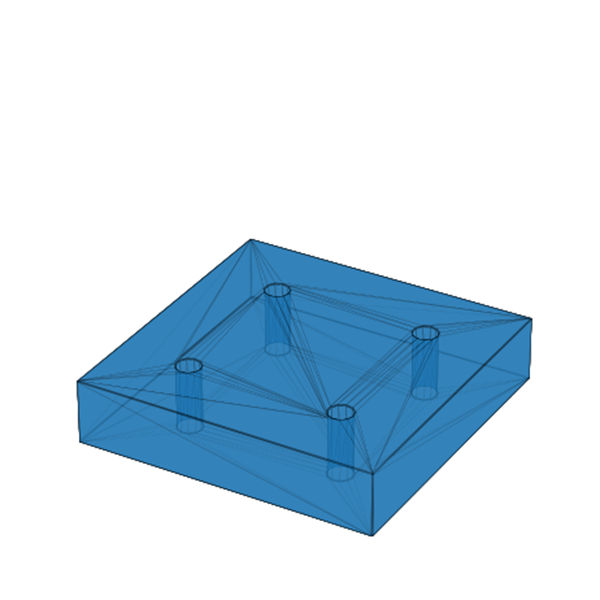
\includegraphics[width=0.5\linewidth]{figures/image.png}
    \caption{Enter Caption}
    \label{fig:placeholder}
\end{figure}

Шаги:

o3d\_bossExtrusion,
o3d\_cutExtrusion,
o3d\_fillet,
o3d\_fillet

cutExtrusion (отверстия):

\begin{figure}
    \centering
    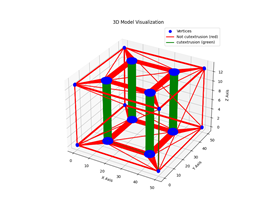
\includegraphics[width=0.5\linewidth]{figures/image2.png}
    \caption{Enter Caption}
    \label{fig:placeholder}
\end{figure}

\begin{figure}
    \centering
    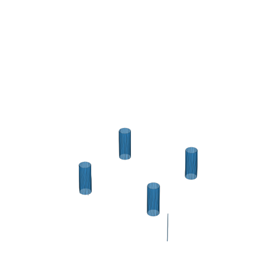
\includegraphics[width=0.5\linewidth]{figures/image3.png}
    \caption{Enter Caption}
    \label{fig:placeholder}
\end{figure}